\documentclass{article}
\usepackage[british]{babel}
\usepackage{meta-inf/lib/naproche}
\documentclass[12pt,oneside]{book}

\usepackage[foundations]{../../lib/tex/naproche}
\usepackage{../../lib/tex/libraries}
\usepackage{graphicx}
\usepackage{float}
\usepackage{caption}
\usepackage{footnote}

\makesavenoteenv{tabular} % Make footnotes work in tabular environments


\title{Foundations of Mathematics}
\author{Marcel Schütz}
\date{2022}

\begin{document}
  \maketitle

  \tableofcontents

  \begin{figure}[H]
    \centering
    \fbox{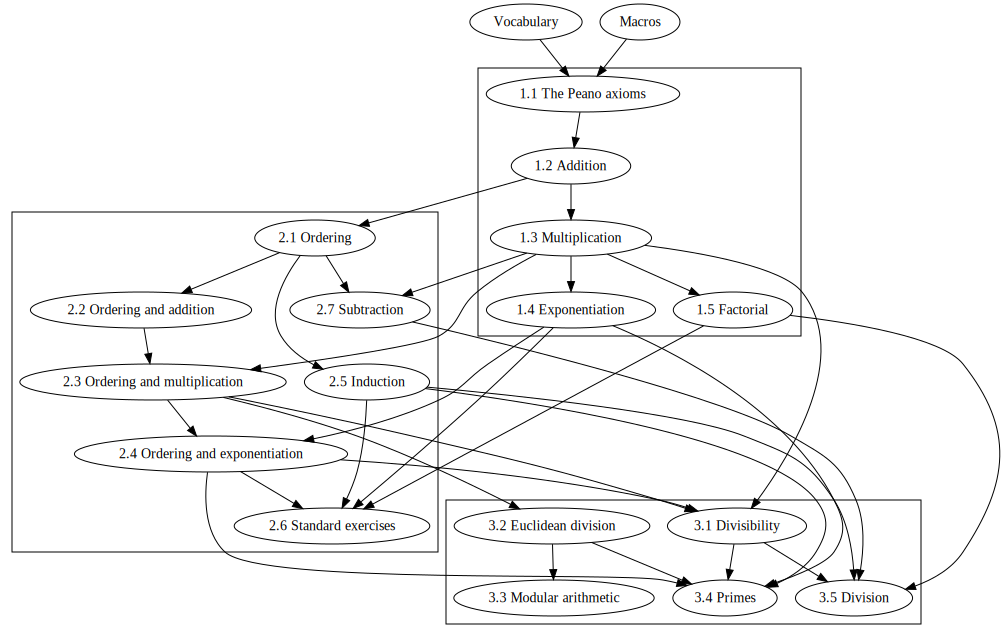
\includegraphics[width=0.9\linewidth]{./dependency-graph/graph.png}}
    \caption*{Interdependencies of the chapters}
  \end{figure}


  \section*{Introduction}

  This is a library providing a foundation of mathematics based on a
  Kelley-Morse like class theory with urelements.
  It introduces common operations on classes like unions or intersections
  (\cref{chapter:classes}) together with detailed proofs of their algebraic
  properties (\cref{chapter:computation-laws-for-classes}), the symmetric
  difference of two classes (\cref{chapter:symmetric-difference}) and the
  notions of ordered pairs and Cartesian products
  (\cref{chapter:pairs-and-products}) as well as proofs of the algebraic
  properties of the latter (\cref{chapter:computation-laws-for-products}).
  Moreover, it provides common operations on maps (\cref{chapter:maps}), various
  properties of images and preimages (\cref{chapter:image-and-preimage}) and the
  notions of injectivity, surjectivity, bijectivity
  (\cref{chapter:injections-surjections-bijections}) and invertibility of maps
  (\cref{chapter:invertible-maps}).
  The library provides an axiom system characterizing sets (\cref{chapter:sets})
  and, furthermore, it covers the notions of binary relations
  (\cref{chapter:binary-relations}), fixed-points of subset preserving maps
  (\cref{chapter:fixed-points}), including and equinumerosity
  (\cref{chapter:equinumerosity}).

  As two famous results it includes the Knaster-Tarski fixed point theorem
  (\cref{FOUNDATIONS_12_8420450166112256}) and the Cantor-Schröder-Bernstein
  theorem (\cref{FOUNDATIONS_13_1913663275401216}).

  \paragraph*{Usage.}
  At the very beginning of each chapter you can find the name of its source
  file, e.g. \path{foundations/sections/01_classes.ftl.tex} for
  \cref{chapter:classes}. This filename can be used to import the chapter via
  \Naproche's \texttt{readtex} instruction to another ForTheL text, e.g.:
  \begin{center}
    \verb`[readtex \path{foundations/sections/01_classes.ftl.tex}]`
  \end{center}

  \paragraph*{Checking times.}
  The checking times for each of the chapters may vary from computer to
  computer, but on mid-range hardware they are likely to be similar to those
  given in table below:

  \begin{center}
    \begin{tabular}{c|c|c}

      & \multicolumn{2}{c}{\textbf{Checking time}}
      \\
      \textbf{Chapter}
      & \textbf{without dependencies}     & \textbf{with dependencies}
      \\ \hline
      \ref{chapter:classes}
      & 00:04 min                         & 00:04 min
      \\
      \ref{chapter:computation-laws-for-classes}
      & 00:12 min                         & 00:16 min
      \\
      \ref{chapter:symmetric-difference}
      & 00:32 min                         & 00:48 min
      \\
      \ref{chapter:pairs-and-products}
      & 00:08 min                         & 00:12 min
      \\
      \ref{chapter:computation-laws-for-products}
      & 01:36 min                         & 01:56 min
      \\
      \ref{chapter:maps}
      & 01:13 min                         & 01:25 min
      \\
      \ref{chapter:image-and-preimage}
      & 01:28 min                         & 02:53 min
      \\
      \ref{chapter:injections-surjections-bijections}
      & 00:38 min                         & 02:03 min
      \\
      \ref{chapter:invertible-maps}
      & 02:20 min                         & 04:23 min
      \\
      \ref{chapter:sets}
      & 02:17 min                         & 06:40 min
      \\
      \ref{chapter:binary-relations}
      & 00:14 min                         & 06:54 min
      \\
      \ref{chapter:fixed-points}
      & 00:33 min                         & 07:13 min
      \\
      \ref{chapter:equinumerosity}
      & 01:48 min                         & 09:01 min
    \end{tabular}
  \end{center}


  \subfile{sections/01_classes.ftl.tex}
  \subfile{sections/02_computation-laws-for-classes.ftl.tex}
  \subfile{sections/03_symmetric-difference.ftl.tex}
  \subfile{sections/04_pairs-and-products.ftl.tex}
  \subfile{sections/05_computation-laws-for-products.ftl.tex}
  \subfile{sections/06_maps.ftl.tex}
  \subfile{sections/07_image-and-preimage.ftl.tex}
  \subfile{sections/08_injections-surjections-bijections.ftl.tex}
  \subfile{sections/09_invertible-maps.ftl.tex}
  \subfile{sections/10_sets.ftl.tex}
  \subfile{sections/11_binary-relations.ftl.tex}
  \subfile{sections/12_fixed-points.ftl.tex}
  \subfile{sections/13_equinumerosity.ftl.tex}
\end{document}

\usepackage{amssymb}

\newcommand{\Nat}{\mathbb{N}}
\newcommand{\Prime}{\mathbb{P}}
\renewcommand{\succ}{\textrm{succ}}
\newcommand{\pred}{\textrm{pred}}
\newcommand{\add}{\textrm{add}}
\newcommand{\mul}{\textrm{mul}}
\renewcommand{\exp}{\textrm{exp}}
\newcommand{\fac}{\textrm{fac}}
\renewcommand{\div}{\mathop{\textrm{div}}}
\renewcommand{\mod}{\mathop{\textrm{mod}}}


\usepackage[backend=bibtex]{biblatex}
\usepackage{csquotes}
\addbibresource{meta-inf/lib/bibliography}

\newcommand{\N}{\mathrm{N}}
\newcommand{\Int}{\mathbb{Z}}
\newcommand{\Ps}{\mathrm{P}}

\title{Furstenberg's proof of the infinitude of primes}
\author{\Naproche formalization:\\[0.5em]Andrei Paskevich, Marcel Schütz}
\date{2024}


\begin{document}
  \maketitle

  \noindent This is a formalization of Furstenberg's topological proof of the
  infinitude of primes \cite[p. 353]{Furstenberg1955}.

  \begin{imports}
    \begin{forthel}
      %[prove off][check off]
      [read \path{libraries/source/arithmetics/primes.ftl.tex}]
      [read \path{libraries/source/arithmetics/nat-is-a-set.ftl.tex}]
      [read \path{libraries/source/set-theory/zf.ftl.tex}]
      [read \path{libraries/source/foundations/closure-under-finite-unions.ftl.tex}]
      %[prove on][check on]
    \end{forthel}
  \end{imports}

  The central idea of Furstenberg's proof is to define a certain topology on
  $\Nat$ from the properties of which we can deduce that the set of
  primes is infinite.\footnote{Actually, Furstenberg's proof makes use of a
  topology on $\Int$. But this topology can as well be restricted to
  $\Nat$ without substantially changing the proof.}

  \begin{forthel}
    Let $n, m, k$ denote natural numbers.
    Let $p, q$ denote nonzero natural numbers.

    \begin{definition}
      Let $A$ be a subset of $\Nat$.
      $A^\complement = \Nat \setminus A$.
    \end{definition}

    Let the complement of $A$ stand for $A^\complement$.

    \begin{lemma}
      The complement of any subset of $\Nat$ is a subset of $\Nat$.
    \end{lemma}
  \end{forthel}

  Towards a suitable topology on $\Nat$ let us define \textit{arithmetic
  sequences} $\N_{n, q}$ on $\Nat$.

  \begin{forthel}
    \begin{definition}
      $\N_{n, q} = \{ m \in \Nat \mid m \equiv n \pmod{q} \}$.
    \end{definition}
  \end{forthel}

  This allows us to define the \textit{evenly spaced natural number
  topology} on $\Nat$, whose open sets are defined as follows.

  \begin{forthel}
    \begin{definition}
      Let $U$ be a subset of $\Nat$.
      $U$ is open iff for any $n \in U$ there exists a $q$ such that
      $\N_{n, q} \subseteq U$.
    \end{definition}

    \begin{definition}
      A system of open sets is a system of sets $S$ such that every element of
      $S$ is an open subset of $\Nat$.
    \end{definition}

    \begin{lemma}
      Every system of open sets is a set.
    \end{lemma}
    \begin{proof}
      Let $S$ be a system of open sets.
      Then $S \subseteq \pow(\Nat)$.
      Hence $S$ is a set.
    \end{proof}
  \end{forthel}

  We can show that the open sets indeed form a topology on $\Nat$.

  \begin{forthel}
    \begin{lemma}
      $\Nat$ and $\emptyset$ are open.
    \end{lemma}

    \begin{lemma}
      Let $U,V$ be open subsets of $\Nat$.
      Then $U \cap V$ is open.
    \end{lemma}
    \begin{proof}
      Let $n \in U \cap V$.
      Take a $q$ such that $\N_{n, q} \subseteq U$.
      Take a $p$ such that $\N_{n, p} \subseteq V$.
      Then $p \cdot q \neq 0$.

      Let us show that $\N_{n, p \cdot q} \subseteq U \cap V$.
        Let $m \in \N_{n, p \cdot q}$.
        We have $m \equiv n \pmod{p \cdot q}$.
        Hence $m \equiv n \pmod{p}$ and $m \equiv n \pmod{q}$.
        Thus $m \in \N_{n, p}$ and $m \in \N_{n, q}$.
        Therefore $m \in U$ and $m \in V$.
        Consequently $m \in U \cap V$.
      End.
    \end{proof}

    \begin{lemma}
      Let $S$ be a system of open sets.
      Then $\bigcup S$ is open.
    \end{lemma}
    \begin{proof}
      Let $n \in \bigcup S$.
      Take a set $M$ such that $n \in M \in S$.
      Consider a $q$ such that $\N_{n, q} \subseteq M$.
      Then $\N_{n, q} \subseteq \bigcup S$.
    \end{proof}
  \end{forthel}

  Now that we have a topology of open sets on $\Nat$, we can continue
  with a characterization of closed sets whose key property is that they are
  closed under finite unions.

  \begin{forthel}
    \begin{definition}
      Let $A$ be a subset of $\Nat$.
      $A$ is closed iff $A^\complement$ is open.
    \end{definition}

    \begin{definition}
      A system of closed sets is a system of sets $S$ such that every element of
      $S$ is a closed subset of $\Nat$.
    \end{definition}

    \begin{lemma}
      Every system of closed sets is a set.
    \end{lemma}
    \begin{proof}
      Let $S$ be a system of closed sets.
      Then $S \subseteq \pow(\Nat)$.
      $\pow(\Nat)$ is a set.
      Hence $S$ is a set.
    \end{proof}

    \begin{lemma}
      Let $S$ be a finite system of closed sets.
      Then $\bigcup S$ is closed.
    \end{lemma}
    \begin{proof}
      Define $C = \{ X \mid X$ is a closed subset of $\Nat \}$.

      Let us show that $A \cup B \in C$ for any $A, B \in C$.
        Let $A, B \in C$.
        Then $A, B$ are closed subsets of $\Nat$.
        We have $((A \cup B)^\complement) = A^\complement \cap B^\complement$. %!
        $A^\complement$ and $B^\complement$ are open.
        Hence $A^\complement \cap B^\complement$ is open.
        Thus $A \cup B$ is a closed subset of $\Nat$.
      End.

      Therefore $C$ is closed under finite unions.
      Consequently $\bigcup S \in C$.
      Indeed $S$ is a subset of $C$.
    \end{proof}
  \end{forthel}

  An important step towards Furstenberg's proof is to show that arithmetic
  sequences are closed.

  \begin{forthel}
    \begin{lemma}
      $\N_{n, q}$ is closed.
    \end{lemma}
    \begin{proof}
      Let $m \in (\N_{n, q})^\complement$.

      Let us show that $\N_{m, q} \subseteq (\N_{n, q})^\complement$.
        Let $k \in \N_{m, q}$.
        Assume $k \notin (\N_{n, q})^\complement$.
        Then $k \equiv m \pmod{q}$ and $n \equiv k \pmod{q}$.
        Hence $m \equiv n \pmod{q}$.
        Therefore $m \in \N_{n, q}$.
        Contradiction.
      End.
    \end{proof}
  \end{forthel}

  Identifying each prime number $p$ with the arithmetic sequence $\N_{0, p}$
  yields a bijection between the set $\Prime$ of all prime numbers and the set
  $\Ps$ of all such sequences $\N_{0, p}$.
  Thus to show that there are infinitely many primes it suffices to show that
  $\Ps$ is infinite.

  \begin{forthel}
    \begin{definition}
      $\Ps = \{ \N_{0, p} \mid p \in \Prime \}$.
    \end{definition}

    \begin{lemma}
      $\Ps$ is a system of closed sets.
    \end{lemma}
    \begin{proof}
      $\N_{0, p}$ is a closed subset of $\Nat$ for every $p \in \Prime$.
    \end{proof}

    \begin{lemma}
      $\Ps$ is a set that is equinumerous to $\Prime$.
    \end{lemma}
    \begin{proof}
      (1) $\Ps$ is a set.
      Indeed $\Ps \subseteq \pow(\Nat)$.

      (2) $\Ps$ is equinumerous to $\Prime$. \\
      Proof.
        Define $f(p) = \N_{0,p}$ for $p \in \Prime$.

        Let us show that $f$ is injective.
          Let $p, q \in \Prime$.
          Assume $f(p) = f(q)$.
          Then $\N_{0, p} = \N_{0, q}$.
          We have $\N_{0, p} = \{ m \in \Nat \mid m \equiv 0 \pmod{p} \}$ and
          $\N_{0, q} = \{ m \in \Nat \mid m \equiv 0 \pmod{q} \}$.

          We can show that for all $m \in \Nat$ we have $p \mid m$ iff $q \mid m$.
            Let $m \in \Nat$.
            Then $m \equiv 0 \pmod{p}$ iff $m \equiv 0 \pmod{q}$.
            Thus $m \mod p = 0 \mod p$ iff $m \mod q = 0 \mod q$.
            We have $0 \mod p = 0 = 0 \mod q$.
            Hence $m \mod p = 0$ iff $m \mod q = 0$.
            Therefore $p \mid m$ iff $q \mid m$.
          End.

          Consequently $p = q$.
        End.

        $f$ is surjective onto $\Ps$.
        Thus $f$ is a bijection between $\Prime$ and $\Ps$.
      Qed.
    \end{proof}

    \begin{theorem}[title=Furstenberg]
      $\Prime$ is infinite.
    \end{theorem}
    \begin{proof}
      $\bigcup \Ps$ is a subset of $\Nat$.

      Let us show that for any $n \in \Nat$ we have $n \in \bigcup \Ps$ iff $n$
      has a prime divisor.
        Let $n \in \Nat$.

        If $n$ has a prime divisor then $n$ belongs to $\bigcup \Ps$. \\
        Proof.
          Assume $n$ has a prime divisor.
          Take a prime divisor $p$ of $n$.
          We have $\N_{0, p} \in \Ps$.
          Hence $n \in \N_{0, p}$.
        Qed.

        If $n$ belongs to $\bigcup \Ps$ then $n$ has a prime divisor. \\
        Proof.
          Assume that $n$ belongs to $\bigcup \Ps$.
          Take a prime number $r$ such that $n \in \N_{0, r}$.
          Hence $n \equiv 0 \pmod{r}$.
          Thus $n \mod r = 0 \mod r = 0$.
          Therefore $r$ is a prime divisor of $n$.
        Qed.
      End.

      Hence For all $n \in \Nat$ we have $n \in (\bigcup \Ps)^\complement$ iff
      $n$ has no prime divisor.
      $1$ has no prime divisor and any natural number having no prime
      divisor is equal to $1$.
      Therefore $(\bigcup \Ps)^\complement = \set{1}$.
      Indeed $((\bigcup \Ps)^\complement) \subseteq \set{1}$ and $\set{1}
      \subseteq (\bigcup \Ps)^\complement$. %!

      $\Ps$ is infinite. \\
      Proof by contradiction.
        Assume that $\Ps$ is finite.
        Then $\bigcup \Ps$ is closed and $(\bigcup \Ps)^\complement$ is open.
        Take a $p$ such that $\N_{1, p} \subseteq (\bigcup \Ps)^\complement$.
        $1 + p$ is an element of $\N_{1, p}$.
        Indeed $1 + p \equiv 1 \pmod{p}$
        (by \printref{ARITHMETIC_08_5984712287846400}).
        $1 + p$ is not equal to $1$.
        Hence $1 + p \notin (\bigcup \Ps)^\complement$.
        Contradiction.
      Qed.
    \end{proof}
  \end{forthel}

  \printbibliography
\end{document}
